\documentclass[1p]{elsarticle_modified}
%\bibliographystyle{elsarticle-num}

%\usepackage[colorlinks]{hyperref}
%\usepackage{abbrmath_seonhwa} %\Abb, \Ascr, \Acal ,\Abf, \Afrak
\usepackage{amsfonts}
\usepackage{amssymb}
\usepackage{amsmath}
\usepackage{amsthm}
\usepackage{scalefnt}
\usepackage{amsbsy}
\usepackage{kotex}
\usepackage{caption}
\usepackage{subfig}
\usepackage{color}
\usepackage{graphicx}
\usepackage{xcolor} %% white, black, red, green, blue, cyan, magenta, yellow
\usepackage{float}
\usepackage{setspace}
\usepackage{hyperref}

\usepackage{tikz}
\usetikzlibrary{arrows}

\usepackage{multirow}
\usepackage{array} % fixed length table
\usepackage{hhline}

%%%%%%%%%%%%%%%%%%%%%
\makeatletter
\renewcommand*\env@matrix[1][\arraystretch]{%
	\edef\arraystretch{#1}%
	\hskip -\arraycolsep
	\let\@ifnextchar\new@ifnextchar
	\array{*\c@MaxMatrixCols c}}
\makeatother %https://tex.stackexchange.com/questions/14071/how-can-i-increase-the-line-spacing-in-a-matrix
%%%%%%%%%%%%%%%

\usepackage[normalem]{ulem}

\newcommand{\msout}[1]{\ifmmode\text{\sout{\ensuremath{#1}}}\else\sout{#1}\fi}
%SOURCE: \msout is \stkout macro in https://tex.stackexchange.com/questions/20609/strikeout-in-math-mode

\newcommand{\cancel}[1]{
	\ifmmode
	{\color{red}\msout{#1}}
	\else
	{\color{red}\sout{#1}}
	\fi
}

\newcommand{\add}[1]{
	{\color{blue}\uwave{#1}}
}

\newcommand{\replace}[2]{
	\ifmmode
	{\color{red}\msout{#1}}{\color{blue}\uwave{#2}}
	\else
	{\color{red}\sout{#1}}{\color{blue}\uwave{#2}}
	\fi
}

\newcommand{\Sol}{\mathcal{S}} %segment
\newcommand{\D}{D} %diagram
\newcommand{\A}{\mathcal{A}} %arc


%%%%%%%%%%%%%%%%%%%%%%%%%%%%%5 test

\def\sl{\operatorname{\textup{SL}}(2,\Cbb)}
\def\psl{\operatorname{\textup{PSL}}(2,\Cbb)}
\def\quan{\mkern 1mu \triangleright \mkern 1mu}

\theoremstyle{definition}
\newtheorem{thm}{Theorem}[section]
\newtheorem{prop}[thm]{Proposition}
\newtheorem{lem}[thm]{Lemma}
\newtheorem{ques}[thm]{Question}
\newtheorem{cor}[thm]{Corollary}
\newtheorem{defn}[thm]{Definition}
\newtheorem{exam}[thm]{Example}
\newtheorem{rmk}[thm]{Remark}
\newtheorem{alg}[thm]{Algorithm}

\newcommand{\I}{\sqrt{-1}}
\begin{document}

%\begin{frontmatter}
%
%\title{Boundary parabolic representations of knots up to 8 crossings}
%
%%% Group authors per affiliation:
%\author{Yunhi Cho} 
%\address{Department of Mathematics, University of Seoul, Seoul, Korea}
%\ead{yhcho@uos.ac.kr}
%
%
%\author{Seonhwa Kim} %\fnref{s_kim}}
%\address{Center for Geometry and Physics, Institute for Basic Science, Pohang, 37673, Korea}
%\ead{ryeona17@ibs.re.kr}
%
%\author{Hyuk Kim}
%\address{Department of Mathematical Sciences, Seoul National University, Seoul 08826, Korea}
%\ead{hyukkim@snu.ac.kr}
%
%\author{Seokbeom Yoon}
%\address{Department of Mathematical Sciences, Seoul National University, Seoul, 08826,  Korea}
%\ead{sbyoon15@snu.ac.kr}
%
%\begin{abstract}
%We find all boundary parabolic representation of knots up to 8 crossings.
%
%\end{abstract}
%\begin{keyword}
%    \MSC[2010] 57M25 
%\end{keyword}
%
%\end{frontmatter}

%\linenumbers
%\tableofcontents
%
\newcommand\colored[1]{\textcolor{white}{\rule[-0.35ex]{0.8em}{1.4ex}}\kern-0.8em\color{red} #1}%
%\newcommand\colored[1]{\textcolor{white}{ #1}\kern-2.17ex	\textcolor{white}{ #1}\kern-1.81ex	\textcolor{white}{ #1}\kern-2.15ex\color{red}#1	}

{\Large $\underline{9_{32}~(K9a_{6})}$}

\setlength{\tabcolsep}{10pt}
\renewcommand{\arraystretch}{1.6}
\vspace{1cm}\begin{tabular}{m{100pt}>{\centering\arraybackslash}m{274pt}}
\multirow{5}{120pt}{
	\centering
	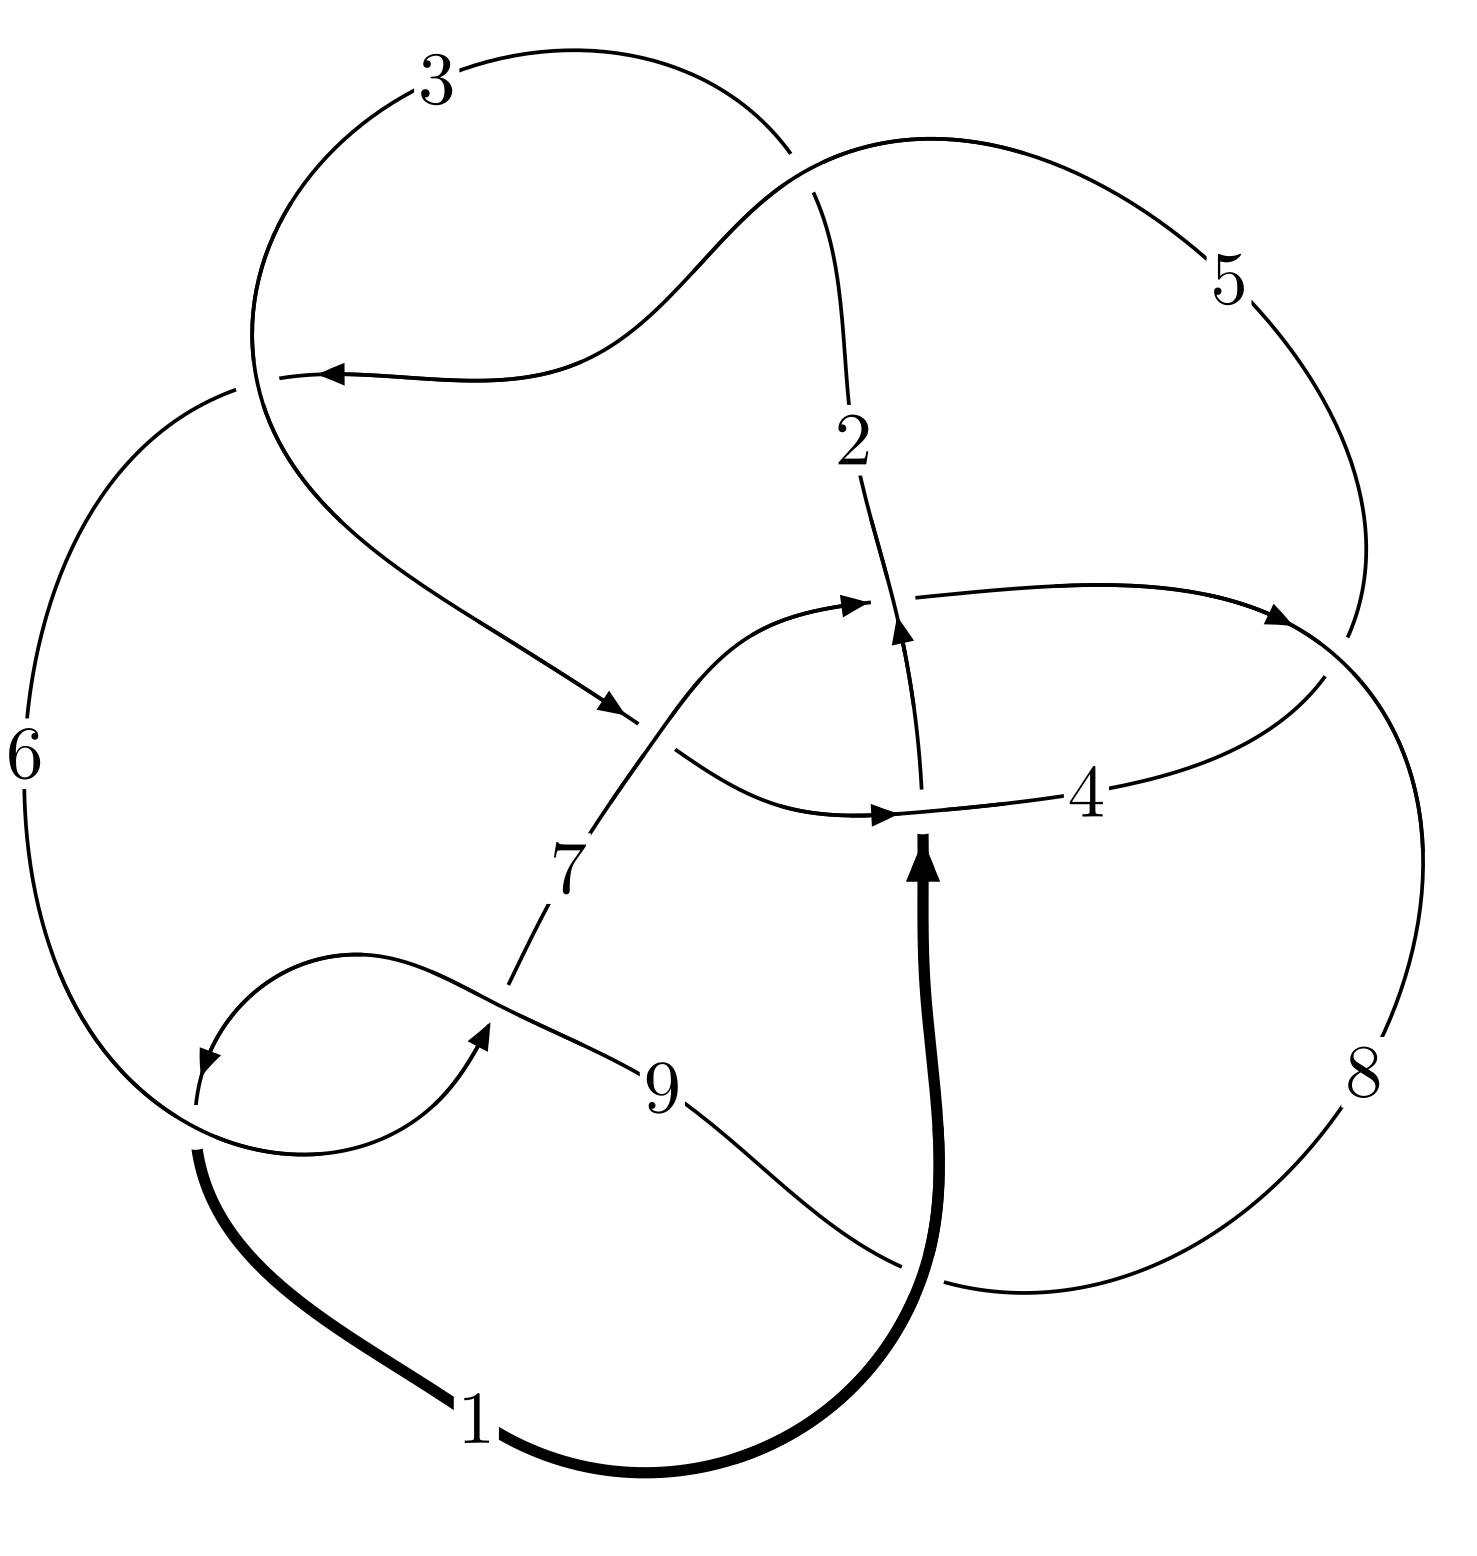
\includegraphics[width=112pt]{../../../GIT/diagram.site/Diagrams/png/67_9_32.png}\\
\ \ \ A knot diagram\footnotemark}&
\allowdisplaybreaks
\textbf{Linearized knot diagam} \\
\cline{2-2}
 &
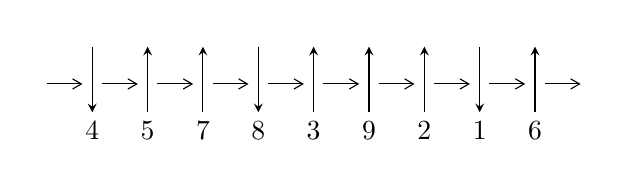
\begin{tikzpicture}[x=20pt, y=17pt]
	% nodes
	\node (C0) at (0, 0) {};
	\node (C1) at (1, 0) {};
	\node (C1U) at (1, +1) {};
	\node (C1D) at (1, -1) {4};

	\node (C2) at (2, 0) {};
	\node (C2U) at (2, +1) {};
	\node (C2D) at (2, -1) {5};

	\node (C3) at (3, 0) {};
	\node (C3U) at (3, +1) {};
	\node (C3D) at (3, -1) {7};

	\node (C4) at (4, 0) {};
	\node (C4U) at (4, +1) {};
	\node (C4D) at (4, -1) {8};

	\node (C5) at (5, 0) {};
	\node (C5U) at (5, +1) {};
	\node (C5D) at (5, -1) {3};

	\node (C6) at (6, 0) {};
	\node (C6U) at (6, +1) {};
	\node (C6D) at (6, -1) {9};

	\node (C7) at (7, 0) {};
	\node (C7U) at (7, +1) {};
	\node (C7D) at (7, -1) {2};

	\node (C8) at (8, 0) {};
	\node (C8U) at (8, +1) {};
	\node (C8D) at (8, -1) {1};

	\node (C9) at (9, 0) {};
	\node (C9U) at (9, +1) {};
	\node (C9D) at (9, -1) {6};
	\node (C10) at (10, 0) {};

	% arrows
	\draw[->,>={angle 60}]
	(C0) edge (C1) (C1) edge (C2) (C2) edge (C3) (C3) edge (C4) (C4) edge (C5) (C5) edge (C6) (C6) edge (C7) (C7) edge (C8) (C8) edge (C9) (C9) edge (C10) ;	\draw[->,>=stealth]
	(C1U) edge (C1D) (C2D) edge (C2U) (C3D) edge (C3U) (C4U) edge (C4D) (C5D) edge (C5U) (C6D) edge (C6U) (C7D) edge (C7U) (C8U) edge (C8D) (C9D) edge (C9U) ;
	\end{tikzpicture} \\
\hhline{~~} \\& 
\textbf{Solving Sequence} \\ \cline{2-2} 
 &
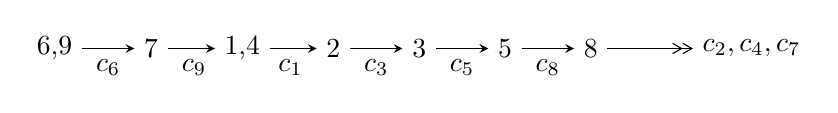
\begin{tikzpicture}[x=31pt, y=7pt]
	% node
	\node (A0) at (-1/8, 0) {6,9};
	\node (A1) at (1, 0) {7};
	\node (A2) at (33/16, 0) {1,4};
	\node (A3) at (25/8, 0) {2};
	\node (A4) at (33/8, 0) {3};
	\node (A5) at (41/8, 0) {5};
	\node (A6) at (49/8, 0) {8};
	\node (C1) at (1/2, -1) {$c_{6}$};
	\node (C2) at (3/2, -1) {$c_{9}$};
	\node (C3) at (21/8, -1) {$c_{1}$};
	\node (C4) at (29/8, -1) {$c_{3}$};
	\node (C5) at (37/8, -1) {$c_{5}$};
	\node (C6) at (45/8, -1) {$c_{8}$};
	\node (A7) at (8, 0) {$c_{2},c_{4},c_{7}$};

	% edge
	\draw[->,>=stealth]	
	(A0) edge (A1) (A1) edge (A2) (A2) edge (A3) (A3) edge (A4) (A4) edge (A5) (A5) edge (A6) ;
	\draw[->>,>={angle 60}]	
	(A6) edge (A7);
\end{tikzpicture} \\ 

\end{tabular} \\

\footnotetext{
The image of knot diagram is generated by the software ``\textbf{Draw programme}" developed by Andrew Bartholomew(\url{http://www.layer8.co.uk/maths/draw/index.htm\#Running-draw}), where we modified some parts for our purpose(\url{https://github.com/CATsTAILs/LinksPainter}).
}\phantom \\ \newline 
\centering \textbf{Ideals for irreducible components\footnotemark of $X_{\text{par}}$} 
 
\begin{align*}
I^u_{1}&=\langle 
216472320 u^{28}-196425840 u^{27}+\cdots+2595371149 b-196454684,\\
\phantom{I^u_{1}}&\phantom{= \langle  }-230172 u^{28}-27804388 u^{27}+\cdots+370767307 a-679741065,\;u^{29}- u^{28}+\cdots+3 u+1\rangle \\
\\
\end{align*}
\raggedright * 1 irreducible components of $\dim_{\mathbb{C}}=0$, with total 29 representations.\\
\footnotetext{All coefficients of polynomials are rational numbers. But the coefficients are sometimes approximated in decimal forms when there is not enough margin.}
\newpage
\renewcommand{\arraystretch}{1}
\centering \section*{I. $I^u_{1}= \langle 2.16\times10^{8} u^{28}-1.96\times10^{8} u^{27}+\cdots+2.60\times10^{9} b-1.96\times10^{8},\;-2.30\times10^{5} u^{28}-2.78\times10^{7} u^{27}+\cdots+3.71\times10^{8} a-6.80\times10^{8},\;u^{29}- u^{28}+\cdots+3 u+1 \rangle$}
\flushleft \textbf{(i) Arc colorings}\\
\begin{tabular}{m{7pt} m{180pt} m{7pt} m{180pt} }
\flushright $a_{6}=$&$\begin{pmatrix}1\\0\end{pmatrix}$ \\
\flushright $a_{9}=$&$\begin{pmatrix}0\\u\end{pmatrix}$ \\
\flushright $a_{7}=$&$\begin{pmatrix}1\\- u^2\end{pmatrix}$ \\
\flushright $a_{1}=$&$\begin{pmatrix}u\\u\end{pmatrix}$ \\
\flushright $a_{4}=$&$\begin{pmatrix}0.000620799 u^{28}+0.0749915 u^{27}+\cdots-3.83846 u+1.83334\\-0.0834071 u^{28}+0.0756831 u^{27}+\cdots-2.93896 u+0.0756943\end{pmatrix}$ \\
\flushright $a_{2}=$&$\begin{pmatrix}-0.00281892 u^{28}-0.833272 u^{27}+\cdots-4.55210 u-0.116626\\0.833292 u^{28}-0.836091 u^{27}+\cdots-3.22782 u-0.836111\end{pmatrix}$ \\
\flushright $a_{3}=$&$\begin{pmatrix}-0.00528313 u^{28}+0.821590 u^{27}+\cdots-0.672045 u+1.83325\\-0.0166708 u^{28}+0.0163909 u^{27}+\cdots-0.722782 u+0.816389\end{pmatrix}$ \\
\flushright $a_{5}=$&$\begin{pmatrix}0.00446172 u^{28}+0.730031 u^{27}+\cdots-2.03460 u+2.48337\\0.0666831 u^{28}-0.0655635 u^{27}+\cdots-1.10887 u+0.734444\end{pmatrix}$ \\
\flushright $a_{8}=$&$\begin{pmatrix}u^3\\u^3+u\end{pmatrix}$\\ \flushright $a_{8}=$&$\begin{pmatrix}u^3\\u^3+u\end{pmatrix}$\\&\end{tabular}
\flushleft \textbf{(ii) Obstruction class $= -1$}\\~\\
\flushleft \textbf{(iii) Cusp Shapes $= -\frac{8357107928}{2595371149} u^{28}+\frac{6279939276}{2595371149} u^{27}+\cdots+\frac{20588201632}{2595371149} u+\frac{13962231674}{2595371149}$}\\~\\
\newpage\renewcommand{\arraystretch}{1}
\flushleft \textbf{(iv) u-Polynomials at the component}\newline \\
\begin{tabular}{m{50pt}|m{274pt}}
Crossings & \hspace{64pt}u-Polynomials at each crossing \\
\hline $$\begin{aligned}c_{1}\end{aligned}$$&$\begin{aligned}
&u^{29}-5 u^{28}+\cdots+u-1
\end{aligned}$\\
\hline $$\begin{aligned}c_{2},c_{5}\end{aligned}$$&$\begin{aligned}
&u^{29}+u^{28}+\cdots+5 u-1
\end{aligned}$\\
\hline $$\begin{aligned}c_{3}\end{aligned}$$&$\begin{aligned}
&u^{29}- u^{28}+\cdots- u-19
\end{aligned}$\\
\hline $$\begin{aligned}c_{4}\end{aligned}$$&$\begin{aligned}
&u^{29}+u^{28}+\cdots+21 u-11
\end{aligned}$\\
\hline $$\begin{aligned}c_{6},c_{9}\end{aligned}$$&$\begin{aligned}
&u^{29}+u^{28}+\cdots+3 u-1
\end{aligned}$\\
\hline $$\begin{aligned}c_{7}\end{aligned}$$&$\begin{aligned}
&u^{29}+3 u^{28}+\cdots+u+1
\end{aligned}$\\
\hline $$\begin{aligned}c_{8}\end{aligned}$$&$\begin{aligned}
&u^{29}+11 u^{28}+\cdots+3 u-1
\end{aligned}$\\
\hline
\end{tabular}\\~\\
\newpage\renewcommand{\arraystretch}{1}
\flushleft \textbf{(v) Riley Polynomials at the component}\newline \\
\begin{tabular}{m{50pt}|m{274pt}}
Crossings & \hspace{64pt}Riley Polynomials at each crossing \\
\hline $$\begin{aligned}c_{1}\end{aligned}$$&$\begin{aligned}
&y^{29}+3 y^{28}+\cdots-5 y-1
\end{aligned}$\\
\hline $$\begin{aligned}c_{2},c_{5}\end{aligned}$$&$\begin{aligned}
&y^{29}-21 y^{28}+\cdots-5 y-1
\end{aligned}$\\
\hline $$\begin{aligned}c_{3}\end{aligned}$$&$\begin{aligned}
&y^{29}+15 y^{28}+\cdots+1103 y-361
\end{aligned}$\\
\hline $$\begin{aligned}c_{4}\end{aligned}$$&$\begin{aligned}
&y^{29}+31 y^{28}+\cdots-1869 y-121
\end{aligned}$\\
\hline $$\begin{aligned}c_{6},c_{9}\end{aligned}$$&$\begin{aligned}
&y^{29}+11 y^{28}+\cdots+3 y-1
\end{aligned}$\\
\hline $$\begin{aligned}c_{7}\end{aligned}$$&$\begin{aligned}
&y^{29}-5 y^{28}+\cdots+3 y-1
\end{aligned}$\\
\hline $$\begin{aligned}c_{8}\end{aligned}$$&$\begin{aligned}
&y^{29}+15 y^{28}+\cdots+175 y-1
\end{aligned}$\\
\hline
\end{tabular}\\~\\
\newpage\flushleft \textbf{(vi) Complex Volumes and Cusp Shapes}
$$\begin{array}{c|c|c}  
\text{Solutions to }I^u_{1}& \I (\text{vol} + \sqrt{-1}CS) & \text{Cusp shape}\\
 \hline 
\begin{aligned}
u &= \phantom{-}0.647818 + 0.782212 I \\
a &= \phantom{-}1.174800 + 0.131909 I \\
b &= \phantom{-}1.35368 - 1.53216 I\end{aligned}
 & \phantom{-}4.48635 + 0.55125 I & \phantom{-}10.94303 - 0.19758 I \\ \hline\begin{aligned}
u &= \phantom{-}0.647818 - 0.782212 I \\
a &= \phantom{-}1.174800 - 0.131909 I \\
b &= \phantom{-}1.35368 + 1.53216 I\end{aligned}
 & \phantom{-}4.48635 - 0.55125 I & \phantom{-}10.94303 + 0.19758 I \\ \hline\begin{aligned}
u &= -0.559219 + 0.861588 I \\
a &= -2.56606 + 1.18824 I \\
b &= -2.19707 + 1.46012 I\end{aligned}
 & \phantom{-}1.99105 - 2.23064 I & -15.0558 - 8.8774 I \\ \hline\begin{aligned}
u &= -0.559219 - 0.861588 I \\
a &= -2.56606 - 1.18824 I \\
b &= -2.19707 - 1.46012 I\end{aligned}
 & \phantom{-}1.99105 + 2.23064 I & -15.0558 + 8.8774 I \\ \hline\begin{aligned}
u &= \phantom{-}0.099472 + 1.040710 I \\
a &= -0.040185 - 0.557055 I \\
b &= -0.559691 + 0.371807 I\end{aligned}
 & -3.62029 - 0.98610 I & -3.43918 + 1.15236 I \\ \hline\begin{aligned}
u &= \phantom{-}0.099472 - 1.040710 I \\
a &= -0.040185 + 0.557055 I \\
b &= -0.559691 - 0.371807 I\end{aligned}
 & -3.62029 + 0.98610 I & -3.43918 - 1.15236 I \\ \hline\begin{aligned}
u &= \phantom{-}0.923879 + 0.554080 I \\
a &= -1.061880 + 0.915307 I \\
b &= \phantom{-}0.170095 + 1.380090 I\end{aligned}
 & \phantom{-}5.89129 - 7.10658 I & \phantom{-}7.40494 + 4.09137 I \\ \hline\begin{aligned}
u &= \phantom{-}0.923879 - 0.554080 I \\
a &= -1.061880 - 0.915307 I \\
b &= \phantom{-}0.170095 - 1.380090 I\end{aligned}
 & \phantom{-}5.89129 + 7.10658 I & \phantom{-}7.40494 - 4.09137 I \\ \hline\begin{aligned}
u &= \phantom{-}0.644129 + 0.902940 I \\
a &= -1.03409 + 1.43901 I \\
b &= \phantom{-}0.565379 + 1.269170 I\end{aligned}
 & \phantom{-}4.11625 + 4.48763 I & \phantom{-}9.60010 - 6.67821 I \\ \hline\begin{aligned}
u &= \phantom{-}0.644129 - 0.902940 I \\
a &= -1.03409 - 1.43901 I \\
b &= \phantom{-}0.565379 - 1.269170 I\end{aligned}
 & \phantom{-}4.11625 - 4.48763 I & \phantom{-}9.60010 + 6.67821 I\\
 \hline 
 \end{array}$$\newpage$$\begin{array}{c|c|c}  
\text{Solutions to }I^u_{1}& \I (\text{vol} + \sqrt{-1}CS) & \text{Cusp shape}\\
 \hline 
\begin{aligned}
u &= -0.528836 + 0.980105 I \\
a &= -0.540279 - 0.869458 I \\
b &= -0.347922 - 1.350220 I\end{aligned}
 & -0.15788 - 2.80514 I & \phantom{-}1.82209 + 1.85203 I \\ \hline\begin{aligned}
u &= -0.528836 - 0.980105 I \\
a &= -0.540279 + 0.869458 I \\
b &= -0.347922 + 1.350220 I\end{aligned}
 & -0.15788 + 2.80514 I & \phantom{-}1.82209 - 1.85203 I \\ \hline\begin{aligned}
u &= -1.034250 + 0.485851 I \\
a &= -0.549331 - 0.039451 I \\
b &= -0.348963 - 0.675392 I\end{aligned}
 & \phantom{-}5.14963 - 1.80223 I & \phantom{-}13.69706 + 3.37820 I \\ \hline\begin{aligned}
u &= -1.034250 - 0.485851 I \\
a &= -0.549331 + 0.039451 I \\
b &= -0.348963 + 0.675392 I\end{aligned}
 & \phantom{-}5.14963 + 1.80223 I & \phantom{-}13.69706 - 3.37820 I \\ \hline\begin{aligned}
u &= \phantom{-}0.641135 + 0.564919 I \\
a &= \phantom{-}1.42824 - 0.88660 I \\
b &= -0.129556 - 1.400390 I\end{aligned}
 & \phantom{-}0.91572 - 2.15286 I & \phantom{-}5.11617 + 3.69479 I \\ \hline\begin{aligned}
u &= \phantom{-}0.641135 - 0.564919 I \\
a &= \phantom{-}1.42824 + 0.88660 I \\
b &= -0.129556 + 1.400390 I\end{aligned}
 & \phantom{-}0.91572 + 2.15286 I & \phantom{-}5.11617 - 3.69479 I \\ \hline\begin{aligned}
u &= -0.447738 + 0.689000 I \\
a &= \phantom{-}1.79794 - 0.28016 I \\
b &= \phantom{-}1.170450 + 0.106145 I\end{aligned}
 & \phantom{-}0.78940 - 1.37762 I & \phantom{-}5.11267 + 4.75149 I \\ \hline\begin{aligned}
u &= -0.447738 - 0.689000 I \\
a &= \phantom{-}1.79794 + 0.28016 I \\
b &= \phantom{-}1.170450 - 0.106145 I\end{aligned}
 & \phantom{-}0.78940 + 1.37762 I & \phantom{-}5.11267 - 4.75149 I \\ \hline\begin{aligned}
u &= \phantom{-}0.618739 + 1.016340 I \\
a &= -1.74109 + 0.57301 I \\
b &= -1.33104 + 1.93207 I\end{aligned}
 & -0.38505 + 7.12556 I & \phantom{-}2.65443 - 8.10425 I \\ \hline\begin{aligned}
u &= \phantom{-}0.618739 - 1.016340 I \\
a &= -1.74109 - 0.57301 I \\
b &= -1.33104 - 1.93207 I\end{aligned}
 & -0.38505 - 7.12556 I & \phantom{-}2.65443 + 8.10425 I\\
 \hline 
 \end{array}$$\newpage$$\begin{array}{c|c|c}  
\text{Solutions to }I^u_{1}& \I (\text{vol} + \sqrt{-1}CS) & \text{Cusp shape}\\
 \hline 
\begin{aligned}
u &= -0.111222 + 1.267020 I \\
a &= -0.303660 + 0.158824 I \\
b &= \phantom{-}0.107002 - 0.499750 I\end{aligned}
 & -1.26594 - 5.18635 I & \phantom{-}1.49328 + 7.03100 I \\ \hline\begin{aligned}
u &= -0.111222 - 1.267020 I \\
a &= -0.303660 - 0.158824 I \\
b &= \phantom{-}0.107002 + 0.499750 I\end{aligned}
 & -1.26594 + 5.18635 I & \phantom{-}1.49328 - 7.03100 I \\ \hline\begin{aligned}
u &= \phantom{-}0.708050 + 1.105240 I \\
a &= \phantom{-}1.56079 - 0.79326 I \\
b &= \phantom{-}1.27636 - 1.94848 I\end{aligned}
 & \phantom{-}4.19521 + 13.09990 I & \phantom{-}5.01719 - 8.12211 I \\ \hline\begin{aligned}
u &= \phantom{-}0.708050 - 1.105240 I \\
a &= \phantom{-}1.56079 + 0.79326 I \\
b &= \phantom{-}1.27636 + 1.94848 I\end{aligned}
 & \phantom{-}4.19521 - 13.09990 I & \phantom{-}5.01719 + 8.12211 I \\ \hline\begin{aligned}
u &= -0.770179 + 1.141350 I \\
a &= \phantom{-}0.718662 + 0.419411 I \\
b &= \phantom{-}0.461012 + 0.914365 I\end{aligned}
 & \phantom{-}3.17430 - 4.69569 I & \phantom{-}8.95566 + 8.13169 I \\ \hline\begin{aligned}
u &= -0.770179 - 1.141350 I \\
a &= \phantom{-}0.718662 - 0.419411 I \\
b &= \phantom{-}0.461012 - 0.914365 I\end{aligned}
 & \phantom{-}3.17430 + 4.69569 I & \phantom{-}8.95566 - 8.13169 I \\ \hline\begin{aligned}
u &= -0.195750 + 0.569252 I \\
a &= \phantom{-}1.95836 - 0.88135 I \\
b &= \phantom{-}0.778642 - 0.497191 I\end{aligned}
 & \phantom{-}0.70687 - 1.36069 I & \phantom{-}4.42210 + 4.47976 I \\ \hline\begin{aligned}
u &= -0.195750 - 0.569252 I \\
a &= \phantom{-}1.95836 + 0.88135 I \\
b &= \phantom{-}0.778642 + 0.497191 I\end{aligned}
 & \phantom{-}0.70687 + 1.36069 I & \phantom{-}4.42210 - 4.47976 I \\ \hline\begin{aligned}
u &= -0.272051\phantom{ +0.000000I} \\
a &= \phantom{-}3.39557\phantom{ +0.000000I} \\
b &= \phantom{-}1.06327\phantom{ +0.000000I}\end{aligned}
 & \phantom{-}2.30899\phantom{ +0.000000I} & \phantom{-}2.51260\phantom{ +0.000000I}\\
 \hline 
 \end{array}$$\newpage
\newpage\renewcommand{\arraystretch}{1}
\centering \section*{ II. u-Polynomials}
\begin{tabular}{m{50pt}|m{274pt}}
Crossings & \hspace{64pt}u-Polynomials at each crossing \\
\hline $$\begin{aligned}c_{1}\end{aligned}$$&$\begin{aligned}
&u^{29}-5 u^{28}+\cdots+u-1
\end{aligned}$\\
\hline $$\begin{aligned}c_{2},c_{5}\end{aligned}$$&$\begin{aligned}
&u^{29}+u^{28}+\cdots+5 u-1
\end{aligned}$\\
\hline $$\begin{aligned}c_{3}\end{aligned}$$&$\begin{aligned}
&u^{29}- u^{28}+\cdots- u-19
\end{aligned}$\\
\hline $$\begin{aligned}c_{4}\end{aligned}$$&$\begin{aligned}
&u^{29}+u^{28}+\cdots+21 u-11
\end{aligned}$\\
\hline $$\begin{aligned}c_{6},c_{9}\end{aligned}$$&$\begin{aligned}
&u^{29}+u^{28}+\cdots+3 u-1
\end{aligned}$\\
\hline $$\begin{aligned}c_{7}\end{aligned}$$&$\begin{aligned}
&u^{29}+3 u^{28}+\cdots+u+1
\end{aligned}$\\
\hline $$\begin{aligned}c_{8}\end{aligned}$$&$\begin{aligned}
&u^{29}+11 u^{28}+\cdots+3 u-1
\end{aligned}$\\
\hline
\end{tabular}\newpage\renewcommand{\arraystretch}{1}
\centering \section*{ III. Riley Polynomials}
\begin{tabular}{m{50pt}|m{274pt}}
Crossings & \hspace{64pt}Riley Polynomials at each crossing \\
\hline $$\begin{aligned}c_{1}\end{aligned}$$&$\begin{aligned}
&y^{29}+3 y^{28}+\cdots-5 y-1
\end{aligned}$\\
\hline $$\begin{aligned}c_{2},c_{5}\end{aligned}$$&$\begin{aligned}
&y^{29}-21 y^{28}+\cdots-5 y-1
\end{aligned}$\\
\hline $$\begin{aligned}c_{3}\end{aligned}$$&$\begin{aligned}
&y^{29}+15 y^{28}+\cdots+1103 y-361
\end{aligned}$\\
\hline $$\begin{aligned}c_{4}\end{aligned}$$&$\begin{aligned}
&y^{29}+31 y^{28}+\cdots-1869 y-121
\end{aligned}$\\
\hline $$\begin{aligned}c_{6},c_{9}\end{aligned}$$&$\begin{aligned}
&y^{29}+11 y^{28}+\cdots+3 y-1
\end{aligned}$\\
\hline $$\begin{aligned}c_{7}\end{aligned}$$&$\begin{aligned}
&y^{29}-5 y^{28}+\cdots+3 y-1
\end{aligned}$\\
\hline $$\begin{aligned}c_{8}\end{aligned}$$&$\begin{aligned}
&y^{29}+15 y^{28}+\cdots+175 y-1
\end{aligned}$\\
\hline
\end{tabular}
\vskip 2pc
\end{document}